\documentclass[12pt,a4paper]{scrartcl}\usepackage[]{graphicx}\usepackage[]{color}
%% maxwidth is the original width if it is less than linewidth
%% otherwise use linewidth (to make sure the graphics do not exceed the margin)
\makeatletter
\def\maxwidth{ %
  \ifdim\Gin@nat@width>\linewidth
    \linewidth
  \else
    \Gin@nat@width
  \fi
}
\makeatother

\definecolor{fgcolor}{rgb}{0.345, 0.345, 0.345}
\newcommand{\hlnum}[1]{\textcolor[rgb]{0.686,0.059,0.569}{#1}}%
\newcommand{\hlstr}[1]{\textcolor[rgb]{0.192,0.494,0.8}{#1}}%
\newcommand{\hlcom}[1]{\textcolor[rgb]{0.678,0.584,0.686}{\textit{#1}}}%
\newcommand{\hlopt}[1]{\textcolor[rgb]{0,0,0}{#1}}%
\newcommand{\hlstd}[1]{\textcolor[rgb]{0.345,0.345,0.345}{#1}}%
\newcommand{\hlkwa}[1]{\textcolor[rgb]{0.161,0.373,0.58}{\textbf{#1}}}%
\newcommand{\hlkwb}[1]{\textcolor[rgb]{0.69,0.353,0.396}{#1}}%
\newcommand{\hlkwc}[1]{\textcolor[rgb]{0.333,0.667,0.333}{#1}}%
\newcommand{\hlkwd}[1]{\textcolor[rgb]{0.737,0.353,0.396}{\textbf{#1}}}%
\let\hlipl\hlkwb

\usepackage{framed}
\makeatletter
\newenvironment{kframe}{%
 \def\at@end@of@kframe{}%
 \ifinner\ifhmode%
  \def\at@end@of@kframe{\end{minipage}}%
  \begin{minipage}{\columnwidth}%
 \fi\fi%
 \def\FrameCommand##1{\hskip\@totalleftmargin \hskip-\fboxsep
 \colorbox{shadecolor}{##1}\hskip-\fboxsep
     % There is no \\@totalrightmargin, so:
     \hskip-\linewidth \hskip-\@totalleftmargin \hskip\columnwidth}%
 \MakeFramed {\advance\hsize-\width
   \@totalleftmargin\z@ \linewidth\hsize
   \@setminipage}}%
 {\par\unskip\endMakeFramed%
 \at@end@of@kframe}
\makeatother

\definecolor{shadecolor}{rgb}{.97, .97, .97}
\definecolor{messagecolor}{rgb}{0, 0, 0}
\definecolor{warningcolor}{rgb}{1, 0, 1}
\definecolor{errorcolor}{rgb}{1, 0, 0}
\newenvironment{knitrout}{}{} % an empty environment to be redefined in TeX

\usepackage{alltt}
\usepackage[utf8]{inputenc}
\usepackage{amsmath}
\usepackage{graphicx}
\usepackage{tikz}
%\usepackage{silence}
\usepackage{mdframed}
%\WarningFilter{mdframed}{You got a bad break}
\usepackage[colorinlistoftodos]{todonotes}
\usepackage{listings}
\usepackage{color}
\colorlet{exampcol}{blue!10}
\usepackage{multicol}
\usepackage{booktabs}


\usepackage{setspace}
%\doublespacing

\usepackage[noanswer]{exercise}%[noanswer]

\usepackage[autostyle, english = american]{csquotes}
\MakeOuterQuote{"}

\usepackage{hyperref}
\hypersetup{
    colorlinks,
    citecolor=black,
    filecolor=black,
    linkcolor=blue,
    urlcolor=black
}

\title{Exercises for progamming with functions}
\date{\today}
\author{Timoth\'ee Bonnet}
\IfFileExists{upquote.sty}{\usepackage{upquote}}{}
\begin{document}



\maketitle

\tableofcontents
\ListOfExerciseInToc
\ExerciseLevelInToc{subsubsection}

\clearpage

\section{Simplest functions}

\begin{Exercise}[difficulty=1, title={Build a first function}]
Write a function that return the product of three arbitrary numbers together (x*y*z) provided by the user.
\end{Exercise}
\begin{Answer}
\begin{knitrout}
\definecolor{shadecolor}{rgb}{0.969, 0.969, 0.969}\color{fgcolor}\begin{kframe}
\begin{alltt}
\hlstd{myfunction} \hlkwb{<-} \hlkwa{function}\hlstd{(}\hlkwc{x}\hlstd{,}\hlkwc{y}\hlstd{,}\hlkwc{z}\hlstd{)\{}
  \hlkwd{return}\hlstd{(x}\hlopt{*}\hlstd{y}\hlopt{*}\hlstd{z)}
\hlstd{\}}
\hlkwd{myfunction}\hlstd{(}\hlnum{100}\hlstd{,}\hlnum{2}\hlstd{,} \hlopt{-}\hlnum{0.005}\hlstd{)}
\end{alltt}
\begin{verbatim}
## [1] -1
\end{verbatim}
\end{kframe}
\end{knitrout}
\end{Answer}

\begin{Exercise}[difficulty=2, title={Multiple values in output}]
Write a function that return the product of three arbitrary numbers together (x*y*z) as well as their sum (x+y+z).
\end{Exercise}
\begin{Answer}
\begin{knitrout}
\definecolor{shadecolor}{rgb}{0.969, 0.969, 0.969}\color{fgcolor}\begin{kframe}
\begin{alltt}
\hlstd{myfunction} \hlkwb{<-} \hlkwa{function}\hlstd{(}\hlkwc{x}\hlstd{,}\hlkwc{y}\hlstd{,}\hlkwc{z}\hlstd{)\{}
  \hlkwd{return}\hlstd{(}\hlkwd{c}\hlstd{(x}\hlopt{*}\hlstd{y}\hlopt{*}\hlstd{z, x}\hlopt{+}\hlstd{y}\hlopt{+}\hlstd{z))}
\hlstd{\}}
\hlkwd{myfunction}\hlstd{(}\hlnum{100}\hlstd{,}\hlnum{2}\hlstd{,} \hlopt{-}\hlnum{0.005}\hlstd{)}
\end{alltt}
\begin{verbatim}
## [1]  -1 102
\end{verbatim}
\end{kframe}
\end{knitrout}
\end{Answer}

\clearpage

\begin{Exercise}[difficulty=2, title={Turning a piece of code into a function}]
In a previous session we wrote the following piece of code to simulate p-values for a random effect in a mixed model:
\begin{knitrout}
\definecolor{shadecolor}{rgb}{0.969, 0.969, 0.969}\color{fgcolor}\begin{kframe}
\begin{alltt}
\hlstd{RandomVariance} \hlkwb{<-} \hlnum{0}
\hlstd{sampsize} \hlkwb{<-} \hlnum{500}
\hlstd{nbblocks} \hlkwb{<-} \hlnum{30}
\hlstd{pvals} \hlkwb{<-} \hlkwd{vector}\hlstd{(}\hlkwc{length} \hlstd{=} \hlnum{1000}\hlstd{)}
\hlstd{altpvals} \hlkwb{<-} \hlkwd{vector}\hlstd{(}\hlkwc{length} \hlstd{=} \hlnum{1000}\hlstd{)}
\hlkwa{for} \hlstd{(i} \hlkwa{in} \hlnum{1}\hlopt{:}\hlnum{1000}\hlstd{)}
\hlstd{\{}
\hlstd{x} \hlkwb{<-} \hlkwd{rnorm}\hlstd{(sampsize,}\hlkwc{mean} \hlstd{=} \hlnum{4}\hlstd{,} \hlkwc{sd}\hlstd{=}\hlnum{0.25}\hlstd{)}
\hlstd{block} \hlkwb{<-} \hlkwd{sample}\hlstd{(}\hlkwc{x} \hlstd{=} \hlnum{1}\hlopt{:}\hlstd{nbblocks,} \hlkwc{size} \hlstd{= sampsize,} \hlkwc{replace} \hlstd{=} \hlnum{TRUE}\hlstd{)}
\hlstd{blockvalues} \hlkwb{<-} \hlkwd{rnorm}\hlstd{(}\hlkwc{n} \hlstd{= nbblocks,} \hlkwc{mean} \hlstd{=} \hlnum{0}\hlstd{,} \hlkwc{sd} \hlstd{=} \hlkwd{sqrt}\hlstd{(RandomVariance))}
\hlstd{y} \hlkwb{<-} \hlnum{8} \hlopt{-} \hlstd{x} \hlopt{+} \hlstd{blockvalues[block]} \hlopt{+} \hlkwd{rnorm}\hlstd{(sampsize,}\hlnum{0}\hlstd{,}\hlnum{1}\hlstd{)}
\hlstd{dat} \hlkwb{<-} \hlkwd{data.frame}\hlstd{(}\hlkwc{response} \hlstd{= y,} \hlkwc{predictor} \hlstd{= x,} \hlkwc{block}\hlstd{=block)}
\hlstd{lm0} \hlkwb{<-} \hlkwd{lm}\hlstd{(response} \hlopt{~} \hlnum{1} \hlopt{+} \hlstd{predictor,} \hlkwc{data}\hlstd{=dat)}
\hlstd{lmm0} \hlkwb{<-} \hlkwd{lmer}\hlstd{(response} \hlopt{~} \hlnum{1} \hlopt{+} \hlstd{predictor} \hlopt{+} \hlstd{(}\hlnum{1}\hlopt{|}\hlstd{block),} \hlkwc{data}\hlstd{=dat )}
\hlstd{(LRT0} \hlkwb{<-} \hlkwd{anova}\hlstd{(lmm0, lm0))} \hlcom{#mixed model must come first!}
\hlstd{pvals[i]} \hlkwb{<-} \hlstd{LRT0}\hlopt{$}\hlstd{`Pr(>Chisq)`[}\hlnum{2}\hlstd{]} \hlcom{# the p-value}
\hlstd{altpvals[i]} \hlkwb{<-} \hlnum{1}\hlopt{-}\hlkwd{pchisq}\hlstd{(LRT0}\hlopt{$}\hlstd{Chisq[}\hlnum{2}\hlstd{],}\hlnum{0.5}\hlstd{)} \hlcom{# a better p-value}
\hlstd{\}}
\hlstd{pvals}
\hlstd{altpvals}
\end{alltt}
\end{kframe}
\end{knitrout}

Turn this into a function were the arguments will let you control:
  \begin{itemize}
    \item The value of the simulated variance (RandomVariance)
    \item The number of simulations (above it is fixed to 1000)
    \item (optionally) The sample size and number of random levels (blocks)
  \end{itemize}
And output:
  \begin{itemize}
    \item A vector of standard p-values from the LRT
    \item (optionally) a vector of "alternative" p-values (from the hand-made Chi-square)
    \item (optionally) histograms of the distribution of p-values
  \end{itemize}

\end{Exercise}
\begin{Answer}
\begin{knitrout}
\definecolor{shadecolor}{rgb}{0.969, 0.969, 0.969}\color{fgcolor}\begin{kframe}
\begin{alltt}
\hlstd{Fpvalsimul} \hlkwb{<-} \hlkwa{function}\hlstd{(}\hlkwc{RandomVariance} \hlstd{=} \hlnum{0}\hlstd{,}
                       \hlkwc{sampsize} \hlstd{=} \hlnum{500}\hlstd{,}
                       \hlkwc{nbblocks} \hlstd{=} \hlnum{30}\hlstd{,}
                       \hlkwc{nsimuls} \hlstd{=} \hlnum{100}\hlstd{)\{}
  \hlkwd{require}\hlstd{(lme4)}
\hlstd{pvals} \hlkwb{<-} \hlkwd{vector}\hlstd{(}\hlkwc{length} \hlstd{= nsimuls)}
\hlstd{altpvals} \hlkwb{<-} \hlkwd{vector}\hlstd{(}\hlkwc{length} \hlstd{= nsimuls)}
\hlkwa{for} \hlstd{(i} \hlkwa{in} \hlnum{1}\hlopt{:}\hlstd{nsimuls)}
\hlstd{\{}
\hlstd{x} \hlkwb{<-} \hlkwd{rnorm}\hlstd{(sampsize,}\hlkwc{mean} \hlstd{=} \hlnum{4}\hlstd{,} \hlkwc{sd}\hlstd{=}\hlnum{0.25}\hlstd{)}
\hlstd{block} \hlkwb{<-} \hlkwd{sample}\hlstd{(}\hlkwc{x} \hlstd{=} \hlnum{1}\hlopt{:}\hlstd{nbblocks,} \hlkwc{size} \hlstd{= sampsize,} \hlkwc{replace} \hlstd{=} \hlnum{TRUE}\hlstd{)}
\hlstd{blockvalues} \hlkwb{<-} \hlkwd{rnorm}\hlstd{(}\hlkwc{n} \hlstd{= nbblocks,} \hlkwc{mean} \hlstd{=} \hlnum{0}\hlstd{,} \hlkwc{sd} \hlstd{=} \hlkwd{sqrt}\hlstd{(RandomVariance))}
\hlstd{y} \hlkwb{<-} \hlnum{8} \hlopt{-} \hlstd{x} \hlopt{+} \hlstd{blockvalues[block]} \hlopt{+} \hlkwd{rnorm}\hlstd{(sampsize,}\hlnum{0}\hlstd{,}\hlnum{1}\hlstd{)}
\hlstd{dat} \hlkwb{<-} \hlkwd{data.frame}\hlstd{(}\hlkwc{response} \hlstd{= y,} \hlkwc{predictor} \hlstd{= x,} \hlkwc{block}\hlstd{=block)}
\hlstd{lm0} \hlkwb{<-} \hlkwd{lm}\hlstd{(response} \hlopt{~} \hlnum{1} \hlopt{+} \hlstd{predictor,} \hlkwc{data}\hlstd{=dat)}
\hlstd{lmm0} \hlkwb{<-} \hlkwd{lmer}\hlstd{(response} \hlopt{~} \hlnum{1} \hlopt{+} \hlstd{predictor} \hlopt{+} \hlstd{(}\hlnum{1}\hlopt{|}\hlstd{block),} \hlkwc{data}\hlstd{=dat )}
\hlstd{(LRT0} \hlkwb{<-} \hlkwd{anova}\hlstd{(lmm0, lm0))} \hlcom{#mixed model must come first!}
\hlstd{pvals[i]} \hlkwb{<-} \hlstd{LRT0}\hlopt{$}\hlstd{`Pr(>Chisq)`[}\hlnum{2}\hlstd{]} \hlcom{# the p-value}
\hlstd{altpvals[i]} \hlkwb{<-} \hlnum{1}\hlopt{-}\hlkwd{pchisq}\hlstd{(LRT0}\hlopt{$}\hlstd{Chisq[}\hlnum{2}\hlstd{],}\hlnum{0.5}\hlstd{)} \hlcom{# a better p-value}
\hlstd{\}}
\hlstd{output} \hlkwb{<-} \hlkwd{list}\hlstd{(}\hlkwc{pvals}\hlstd{=pvals,} \hlkwc{altpvals}\hlstd{=altpvals)}
\hlkwd{par}\hlstd{(}\hlkwc{mfrow}\hlstd{=}\hlkwd{c}\hlstd{(}\hlnum{1}\hlstd{,}\hlnum{2}\hlstd{))}
\hlkwd{hist}\hlstd{(pvals);} \hlkwd{hist}\hlstd{(altpvals)}
\hlkwd{return}\hlstd{(output)}
\hlstd{\}}
\end{alltt}
\end{kframe}
\end{knitrout}
\end{Answer}


\clearpage

\begin{Exercise}[difficulty=2, title={Recover the central-limit theorem}]
To simplify, the central-limit theorem states that the sum of independent random distributions tends towards a normal distribution even if the original distributions are non-normal.
Let's write a function that shows that by randomly drawing distributions with random parameters, summing them, and comparing the sum to a Gaussian distribution of same mean and variance.

We can start from the following piece of code:
\begin{knitrout}
\definecolor{shadecolor}{rgb}{0.969, 0.969, 0.969}\color{fgcolor}\begin{kframe}
\begin{alltt}
\hlcom{#how many numbers per distribution:}
\hlstd{n}\hlkwb{=}\hlnum{2000}

\hlcom{# where we will save the sum of distributions:}
\hlstd{output} \hlkwb{<-} \hlkwd{vector}\hlstd{(}\hlkwc{length} \hlstd{= n)}

\hlcom{# three possible distributions to draw from:}
\hlstd{rddistri} \hlkwb{<-} \hlkwd{list}\hlstd{(rnorm,runif,rpois)}

\hlcom{# drawing one number at random to tell which distribution we use:}
\hlstd{choosedistri} \hlkwb{<-} \hlkwd{sample}\hlstd{(}\hlnum{1}\hlopt{:}\hlkwd{length}\hlstd{(rddistri),} \hlkwc{size} \hlstd{=} \hlnum{1}\hlstd{)}
\hlcom{# a trouble is that the different distributions do not take the }
\hlcom{#same number or type of arguments, so we need to have a special}
\hlcom{#piece of code for each of them. For example, for the normal}
\hlcom{#distribution (rnorm):}
\hlkwa{if}\hlstd{(choosedistri}\hlopt{==}\hlnum{1}\hlstd{)}
\hlstd{\{}
    \hlcom{# Decide how you want to select mean and sd:}
     \hlstd{output} \hlkwb{<-} \hlstd{output} \hlopt{+} \hlstd{rddistri[[choosedistri]](n,} \hlkwc{mean}\hlstd{=,} \hlkwc{sd}\hlstd{=)}
\hlstd{\}}
\hlstd{...}
\end{alltt}
\end{kframe}
\end{knitrout}

We may want to use a for loop. We could include also a plot or a statistical test (e.g., shapiro.test).
\end{Exercise}
\begin{Answer}
\begin{knitrout}
\definecolor{shadecolor}{rgb}{0.969, 0.969, 0.969}\color{fgcolor}\begin{kframe}
\begin{alltt}
\hlstd{simclt} \hlkwb{<-} \hlkwa{function}\hlstd{(}\hlkwc{n}\hlstd{=}\hlnum{2000}\hlstd{,} \hlkwc{nbdistri}\hlstd{=}\hlnum{100}\hlstd{)}
\hlstd{\{}
  \hlstd{output} \hlkwb{<-} \hlkwd{vector}\hlstd{(}\hlkwc{length} \hlstd{= n)}
  \hlstd{rddistri} \hlkwb{<-} \hlkwd{list}\hlstd{(rnorm, runif, rpois)}

    \hlkwa{for} \hlstd{(i} \hlkwa{in} \hlnum{1}\hlopt{:}\hlstd{nbdistri)}
  \hlstd{\{}
    \hlstd{choosedistri} \hlkwb{<-} \hlkwd{sample}\hlstd{(}\hlnum{1}\hlopt{:}\hlkwd{length}\hlstd{(rddistri),} \hlkwc{size} \hlstd{=} \hlnum{1}\hlstd{)}
    \hlkwa{if}\hlstd{(choosedistri} \hlopt \hlnum{1}\hlstd{)}
    \hlstd{\{}
      \hlstd{output} \hlkwb{<-} \hlstd{output} \hlopt{+} \hlstd{rddistri[[choosedistri]](n,} \hlkwd{rnorm}\hlstd{(}\hlnum{1}\hlstd{),} \hlkwd{runif}\hlstd{(}\hlnum{1}\hlstd{,}\hlnum{0}\hlstd{,}\hlnum{1}\hlstd{))}
    \hlstd{\}}
    \hlkwa{if}\hlstd{(choosedistri} \hlopt \hlnum{2}\hlstd{)}
    \hlstd{\{}
      \hlstd{output} \hlkwb{<-} \hlstd{output} \hlopt{+} \hlstd{rddistri[[choosedistri]](n,} \hlnum{0}\hlstd{,} \hlkwd{runif}\hlstd{(}\hlnum{1}\hlstd{,}\hlnum{0.1}\hlstd{,}\hlnum{3}\hlstd{))}
    \hlstd{\}}
    \hlkwa{if}\hlstd{(choosedistri} \hlopt \hlnum{3}\hlstd{)}
    \hlstd{\{}
      \hlstd{output} \hlkwb{<-} \hlstd{output} \hlopt{+} \hlstd{rddistri[[choosedistri]](n,} \hlkwd{exp}\hlstd{(}\hlkwd{runif}\hlstd{(}\hlnum{1}\hlstd{)))}
    \hlstd{\}}
  \hlstd{\}}
  \hlkwd{plot}\hlstd{(}\hlkwd{density}\hlstd{(output))}
  \hlkwd{lines}\hlstd{(}\hlkwc{x}\hlstd{=}\hlkwd{seq}\hlstd{(}\hlkwd{min}\hlstd{(output),}\hlkwd{max}\hlstd{(output),}\hlkwc{by} \hlstd{=} \hlnum{1}\hlstd{),} \hlkwc{y}\hlstd{=}\hlkwd{dnorm}\hlstd{(}\hlkwd{seq}\hlstd{(}\hlkwd{min}\hlstd{(output),}\hlkwd{max}\hlstd{(output),}\hlkwc{by} \hlstd{=} \hlnum{1}\hlstd{),} \hlkwc{mean} \hlstd{=} \hlkwd{mean}\hlstd{(output),} \hlkwc{sd}\hlstd{=}\hlkwd{sd}\hlstd{(output)),} \hlkwc{col}\hlstd{=}\hlstr{"red"}\hlstd{)}
  \hlkwd{legend}\hlstd{(}\hlkwc{x}\hlstd{=}\hlstr{"topright"}\hlstd{,} \hlkwc{legend} \hlstd{=} \hlkwd{c}\hlstd{(}\hlstr{"simulation"}\hlstd{,} \hlstr{"Normal distribution"}\hlstd{),} \hlkwc{col}\hlstd{=}\hlkwd{c}\hlstd{(}\hlstr{"black"}\hlstd{,} \hlstr{"red"}\hlstd{),} \hlkwc{lwd}\hlstd{=}\hlnum{1}\hlstd{)}
  \hlkwd{return}\hlstd{(output)}
\hlstd{\}}

\hlstd{res} \hlkwb{<-} \hlkwd{simclt}\hlstd{()}
\end{alltt}
\end{kframe}
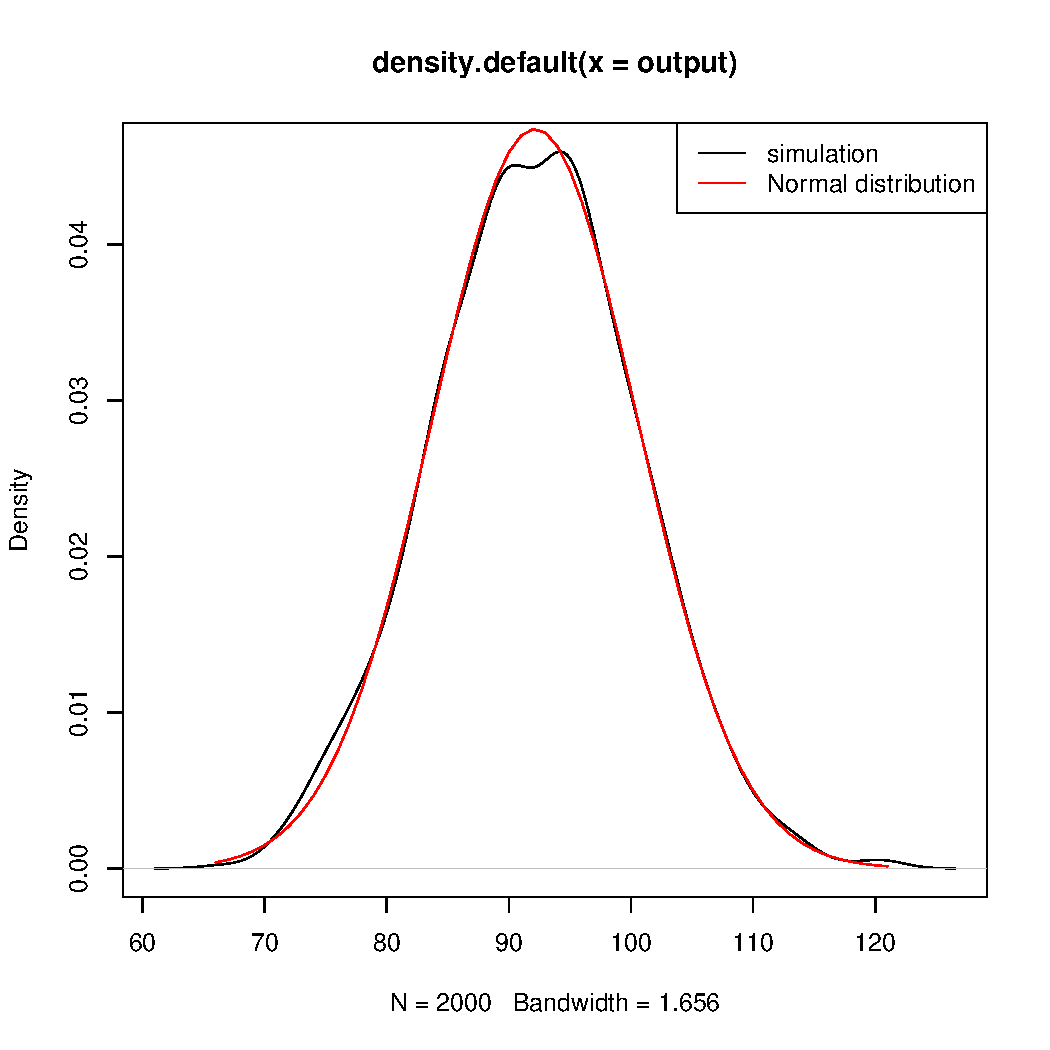
\includegraphics[width=\maxwidth]{figure/unnamed-chunk-7-1} 
\begin{kframe}\begin{alltt}
\hlkwd{shapiro.test}\hlstd{(res)}
\end{alltt}
\begin{verbatim}
## 
## 	Shapiro-Wilk normality test
## 
## data:  res
## W = 1, p-value = 0.4
\end{verbatim}
\end{kframe}
\end{knitrout}
\end{Answer}

\section{Funny things}


\subsection{The dot-dot-dot}

\begin{Exercise}[difficulty=1, title={Understand the \texttt{\dots}}]
Consider these two functions:
\begin{knitrout}
\definecolor{shadecolor}{rgb}{0.969, 0.969, 0.969}\color{fgcolor}\begin{kframe}
\begin{alltt}
\hlstd{halfmean1} \hlkwb{<-} \hlkwa{function}\hlstd{(}\hlkwc{x}\hlstd{)}
\hlstd{\{}
  \hlkwd{mean}\hlstd{(x)}\hlopt{/}\hlnum{2}
\hlstd{\}}
\hlstd{halfmean2} \hlkwb{<-} \hlkwa{function}\hlstd{(}\hlkwc{x}\hlstd{,}\hlkwc{...}\hlstd{)}
\hlstd{\{}
  \hlkwd{mean}\hlstd{(x,...)}\hlopt{/}\hlnum{2}
\hlstd{\}}
\end{alltt}
\end{kframe}
\end{knitrout}

They behave the same way in the first case, but differently in the second:
\begin{knitrout}
\definecolor{shadecolor}{rgb}{0.969, 0.969, 0.969}\color{fgcolor}\begin{kframe}
\begin{alltt}
\hlstd{somedata} \hlkwb{<-} \hlkwd{c}\hlstd{(}\hlnum{10}\hlstd{,} \hlnum{25}\hlstd{,} \hlnum{NA}\hlstd{)}

\hlkwd{halfmean1}\hlstd{(somedata)}
\end{alltt}
\begin{verbatim}
## [1] NA
\end{verbatim}
\begin{alltt}
\hlkwd{halfmean2}\hlstd{(somedata)}
\end{alltt}
\begin{verbatim}
## [1] NA
\end{verbatim}
\begin{alltt}
\hlkwd{halfmean1}\hlstd{(somedata,} \hlkwc{na.rm}\hlstd{=}\hlnum{TRUE}\hlstd{)}
\end{alltt}


{\ttfamily\noindent\bfseries\color{errorcolor}{\#\# Error in halfmean1(somedata, na.rm = TRUE): unused argument (na.rm = TRUE)}}\begin{alltt}
\hlkwd{halfmean2}\hlstd{(somedata,} \hlkwc{na.rm}\hlstd{=}\hlnum{TRUE}\hlstd{)}
\end{alltt}
\begin{verbatim}
## [1] 8.75
\end{verbatim}
\end{kframe}
\end{knitrout}
What does \dots do?
\end{Exercise}
\begin{Answer}
\dots let you pass extra arguments to the function inside your function (but the extra arguments are passed to ALL functions inside, so be careful!)
\end{Answer}

\subsection{The \texttt{<<-} operator}

\begin{Exercise}[difficulty=1, title={Understand the \texttt{<<-}}]
We create to almost identical functions, f0 and f1 and add their output to an object \texttt{x}. Compare the output and explain what happens. What does \texttt{<<-} mean?

\begin{knitrout}
\definecolor{shadecolor}{rgb}{0.969, 0.969, 0.969}\color{fgcolor}\begin{kframe}
\begin{alltt}
\hlstd{f0} \hlkwb{<-} \hlkwa{function}\hlstd{(}\hlkwc{x}\hlstd{=}\hlnum{2}\hlstd{)\{}
  \hlstd{x} \hlkwb{<-} \hlstd{x}
  \hlstd{y} \hlkwb{<-} \hlstd{x}\hlopt{+}\hlnum{2}
  \hlkwd{return}\hlstd{(y)}
\hlstd{\}}

\hlstd{f1} \hlkwb{<-} \hlkwa{function}\hlstd{(}\hlkwc{x}\hlstd{=}\hlnum{2}\hlstd{)\{}
  \hlstd{x} \hlkwb{<<-} \hlstd{x}
  \hlstd{y} \hlkwb{<-} \hlstd{x}\hlopt{+}\hlnum{2}
  \hlkwd{return}\hlstd{(y)}
\hlstd{\}}

\hlstd{x} \hlkwb{<-} \hlkwd{rnorm}\hlstd{(}\hlnum{1000}\hlstd{)}
\hlkwd{f0}\hlstd{()}\hlopt{+}\hlstd{x}

\hlstd{x} \hlkwb{<-} \hlkwd{rnorm}\hlstd{(}\hlnum{1000}\hlstd{)}
\hlkwd{f1}\hlstd{()}\hlopt{+}\hlstd{x}
\end{alltt}
\end{kframe}
\end{knitrout}

\end{Exercise}

\begin{Answer}
The \texttt{<<-} operator breaks the borders of the function environment to assign a value to an object outside that function.
\end{Answer}


\subsection{Recursive functions}

\begin{Exercise}[difficulty=2, title={What does this function do?}]
Consider the following function and try to understand what it does. (code by Dr. Koen van Benthem)
\begin{knitrout}
\definecolor{shadecolor}{rgb}{0.969, 0.969, 0.969}\color{fgcolor}\begin{kframe}
\begin{alltt}
\hlstd{tree}\hlkwb{<-}\hlkwa{function}\hlstd{(}\hlkwc{x}\hlstd{,}\hlkwc{y}\hlstd{,}\hlkwc{l}\hlstd{,}\hlkwc{dir}\hlstd{,}\hlkwc{n}\hlstd{,}\hlkwc{nmax}\hlstd{)\{}
\hlkwa{if}\hlstd{(n}\hlopt{==}\hlnum{0}\hlstd{)\{}
\hlkwd{return}\hlstd{()}
\hlstd{\}}
\hlstd{pos}\hlkwb{<-}\hlkwd{round}\hlstd{(}\hlkwd{runif}\hlstd{(}\hlnum{1}\hlstd{,}\hlnum{1}\hlstd{,}\hlnum{199}\hlstd{))}
\hlstd{colour}\hlkwb{=}\hlkwd{rainbow}\hlstd{(}\hlnum{200}\hlstd{,}\hlkwc{start}\hlstd{=}\hlnum{0.2}\hlstd{,}\hlkwc{end}\hlstd{=}\hlnum{0.6}\hlstd{,}\hlkwc{v}\hlstd{=}\hlnum{0.6}\hlstd{)[pos]}
\hlkwd{lines}\hlstd{(}\hlkwd{c}\hlstd{(x,x}\hlopt{+}\hlstd{l}\hlopt{*}\hlkwd{sin}\hlstd{(dir)),}\hlkwd{c}\hlstd{(y,y}\hlopt{+}\hlstd{l}\hlopt{*}\hlkwd{cos}\hlstd{(dir)),}
      \hlkwc{lwd}\hlstd{=}\hlnum{20}\hlopt{*}\hlstd{(n}\hlopt{/}\hlstd{nmax),}\hlkwc{col}\hlstd{=colour)}
\hlstd{branches}\hlkwb{<-}\hlkwd{round}\hlstd{(}\hlkwd{runif}\hlstd{(}\hlnum{1}\hlstd{,}\hlnum{2}\hlstd{,}\hlnum{4}\hlstd{))}
\hlkwa{for}\hlstd{(i} \hlkwa{in} \hlnum{1}\hlopt{:}\hlstd{branches)\{}
\hlstd{angle}\hlkwb{<-}\hlstd{dir}\hlopt{+}\hlstd{(}\hlopt{-}\hlstd{pi}\hlopt{/}\hlnum{6}\hlstd{)}\hlopt{+}\hlstd{(pi}\hlopt{/}\hlnum{3}\hlstd{)}\hlopt{*}\hlstd{(i}\hlopt{-}\hlnum{1}\hlstd{)}\hlopt{/}\hlstd{(branches}\hlopt{-}\hlnum{1}\hlstd{)}
\hlstd{l2}\hlkwb{<-}\hlkwd{runif}\hlstd{(}\hlnum{1}\hlstd{,}\hlnum{0.7}\hlstd{,}\hlnum{0.85}\hlstd{)}\hlopt{*}\hlstd{l}
\hlkwd{tree}\hlstd{(x}\hlopt{+}\hlstd{l}\hlopt{*}\hlkwd{sin}\hlstd{(dir),y}\hlopt{+}\hlstd{l}\hlopt{*}\hlkwd{cos}\hlstd{(dir),l2,angle,n}\hlopt{-}\hlnum{1}\hlstd{,nmax)}
\hlstd{\}}
\hlstd{\}}
\end{alltt}
\end{kframe}
\end{knitrout}

You can run the function and see if you had guessed right:
\begin{knitrout}
\definecolor{shadecolor}{rgb}{0.969, 0.969, 0.969}\color{fgcolor}\begin{kframe}
\begin{alltt}
\hlkwd{plot}\hlstd{(}\hlnum{0}\hlstd{,}\hlnum{0}\hlstd{,}\hlkwc{type}\hlstd{=}\hlstr{"n"}\hlstd{,}\hlkwc{xlim}\hlstd{=}\hlkwd{c}\hlstd{(}\hlopt{-}\hlnum{10}\hlstd{,}\hlnum{10}\hlstd{),}\hlkwc{ylim}\hlstd{=}\hlkwd{c}\hlstd{(}\hlnum{0}\hlstd{,}\hlnum{10}\hlstd{),}
\hlkwc{xaxt}\hlstd{=}\hlstr{"n"}\hlstd{,}\hlkwc{yaxt}\hlstd{=}\hlstr{"n"}\hlstd{,}\hlkwc{ylab}\hlstd{=}\hlstr{""}\hlstd{,}\hlkwc{xlab}\hlstd{=}\hlstr{""}\hlstd{)}

\hlkwd{tree}\hlstd{(}\hlnum{0}\hlstd{,}\hlnum{0}\hlstd{,}\hlnum{2}\hlstd{,}\hlnum{0}\hlstd{,}\hlnum{8}\hlstd{,}\hlnum{12}\hlstd{)}
\end{alltt}
\end{kframe}
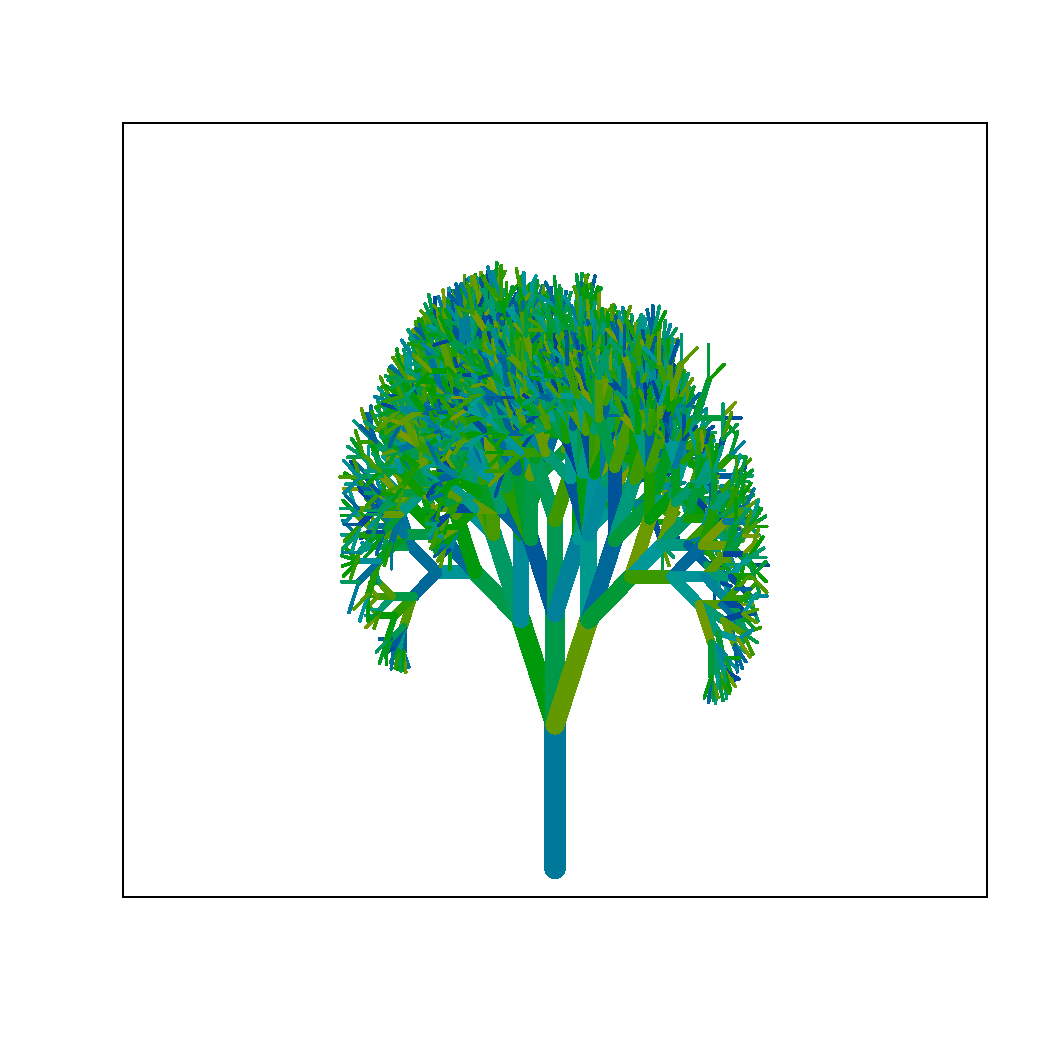
\includegraphics[width=\maxwidth]{figure/unnamed-chunk-12-1} 

\end{knitrout}

What is special about this function? Why should you be careful not to give large values to the parameters n? 
\end{Exercise}
\begin{Answer}
This is a self-referencing function, it calls itself! Each call to the function produces several new calls to the function, and so the number of times the function is called grows exponentially with the value of n. I do not recommend values above 12. That is a general problem to consider with recursive functions. 
\begin{knitrout}
\definecolor{shadecolor}{rgb}{0.969, 0.969, 0.969}\color{fgcolor}\begin{kframe}
\begin{alltt}
\hlstd{tree}\hlkwb{<-}\hlkwa{function}\hlstd{(}\hlkwc{x}\hlstd{,}\hlkwc{y}\hlstd{,}\hlkwc{l}\hlstd{,}\hlkwc{dir}\hlstd{,}\hlkwc{n}\hlstd{,}\hlkwc{nmax}\hlstd{)\{} \hlcom{# We define a function 'tree()'}
\hlcom{# x,y: start of tree, l: length of first branch, dir: direction}
\hlcom{# n and nmax: should be the same number: number of levels in the}
\hlcom{# tree.}
\hlcom{# An important escape argument, leave this out and the function}
\hlcom{# will run forever:}
\hlkwa{if}\hlstd{(n}\hlopt{==}\hlnum{0}\hlstd{)\{}
\hlkwd{return}\hlstd{()}
\hlstd{\}}
\hlcom{# Picking a colour at random using the rainbow function}
\hlcom{# (without this the code would also work, there would just be}
\hlcom{# no colors)}
\hlstd{pos}\hlkwb{<-}\hlkwd{round}\hlstd{(}\hlkwd{runif}\hlstd{(}\hlnum{1}\hlstd{,}\hlnum{1}\hlstd{,}\hlnum{199}\hlstd{))}
\hlstd{colour}\hlkwb{=}\hlkwd{rainbow}\hlstd{(}\hlnum{200}\hlstd{,}\hlkwc{start}\hlstd{=}\hlnum{0.2}\hlstd{,}\hlkwc{end}\hlstd{=}\hlnum{0.6}\hlstd{,}\hlkwc{v}\hlstd{=}\hlnum{0.6}\hlstd{)[pos]}
\hlcom{# Draw a line starting a (x,y) with length 'l' and in direction}
\hlcom{# (in radials) dir. On top of that, we make the width of the}
\hlcom{# line depend on how far the branch is from the stem.}
\hlkwd{lines}\hlstd{(}\hlkwd{c}\hlstd{(x,x}\hlopt{+}\hlstd{l}\hlopt{*}\hlkwd{sin}\hlstd{(dir)),}\hlkwd{c}\hlstd{(y,y}\hlopt{+}\hlstd{l}\hlopt{*}\hlkwd{cos}\hlstd{(dir)),}
      \hlkwc{lwd}\hlstd{=}\hlnum{20}\hlopt{*}\hlstd{(n}\hlopt{/}\hlstd{nmax),}\hlkwc{col}\hlstd{=colour)}
\hlcom{# Generate a random number that defines how many branches the}
\hlcom{# tree has at this point in the structure}
\hlstd{branches}\hlkwb{<-}\hlkwd{round}\hlstd{(}\hlkwd{runif}\hlstd{(}\hlnum{1}\hlstd{,}\hlnum{2}\hlstd{,}\hlnum{4}\hlstd{))}
\hlcom{# Now we go over the separate branches}
\hlkwa{for}\hlstd{(i} \hlkwa{in} \hlnum{1}\hlopt{:}\hlstd{branches)\{}
\hlcom{# to make sure not all branches point in the same direction,}
\hlcom{# we calculate a direction for the branch}
\hlstd{angle}\hlkwb{<-}\hlstd{dir}\hlopt{+}\hlstd{(}\hlopt{-}\hlstd{pi}\hlopt{/}\hlnum{6}\hlstd{)}\hlopt{+}\hlstd{(pi}\hlopt{/}\hlnum{3}\hlstd{)}\hlopt{*}\hlstd{(i}\hlopt{-}\hlnum{1}\hlstd{)}\hlopt{/}\hlstd{(branches}\hlopt{-}\hlnum{1}\hlstd{)}
\hlcom{# Also, we would like the later branches to be smaller than}
\hlcom{# the first one:}
\hlstd{l2}\hlkwb{<-}\hlkwd{runif}\hlstd{(}\hlnum{1}\hlstd{,}\hlnum{0.7}\hlstd{,}\hlnum{0.85}\hlstd{)}\hlopt{*}\hlstd{l}
\hlcom{# And finally the magic of recursion, we draw the new branch}
\hlcom{# simply by using theexact same function: the function 'tree'.}
\hlkwd{tree}\hlstd{(x}\hlopt{+}\hlstd{l}\hlopt{*}\hlkwd{sin}\hlstd{(dir),y}\hlopt{+}\hlstd{l}\hlopt{*}\hlkwd{cos}\hlstd{(dir),l2,angle,n}\hlopt{-}\hlnum{1}\hlstd{,nmax)}
\hlstd{\}}
\hlstd{\}}
\hlcom{# Now, to actually draw the tree, we first make an empty plot}
\hlkwd{plot}\hlstd{(}\hlnum{0}\hlstd{,}\hlnum{0}\hlstd{,}\hlkwc{type}\hlstd{=}\hlstr{"n"}\hlstd{,}\hlkwc{xlim}\hlstd{=}\hlkwd{c}\hlstd{(}\hlopt{-}\hlnum{10}\hlstd{,}\hlnum{10}\hlstd{),}\hlkwc{ylim}\hlstd{=}\hlkwd{c}\hlstd{(}\hlnum{0}\hlstd{,}\hlnum{10}\hlstd{),}
\hlkwc{xaxt}\hlstd{=}\hlstr{"n"}\hlstd{,}\hlkwc{yaxt}\hlstd{=}\hlstr{"n"}\hlstd{,}\hlkwc{ylab}\hlstd{=}\hlstr{""}\hlstd{,}\hlkwc{xlab}\hlstd{=}\hlstr{""}\hlstd{)}
\hlcom{# And then call the function tree() with the parameters we like}
\hlkwd{tree}\hlstd{(}\hlnum{0}\hlstd{,}\hlnum{0}\hlstd{,}\hlnum{2}\hlstd{,}\hlnum{0}\hlstd{,}\hlnum{8}\hlstd{,}\hlnum{8}\hlstd{)}
\end{alltt}
\end{kframe}
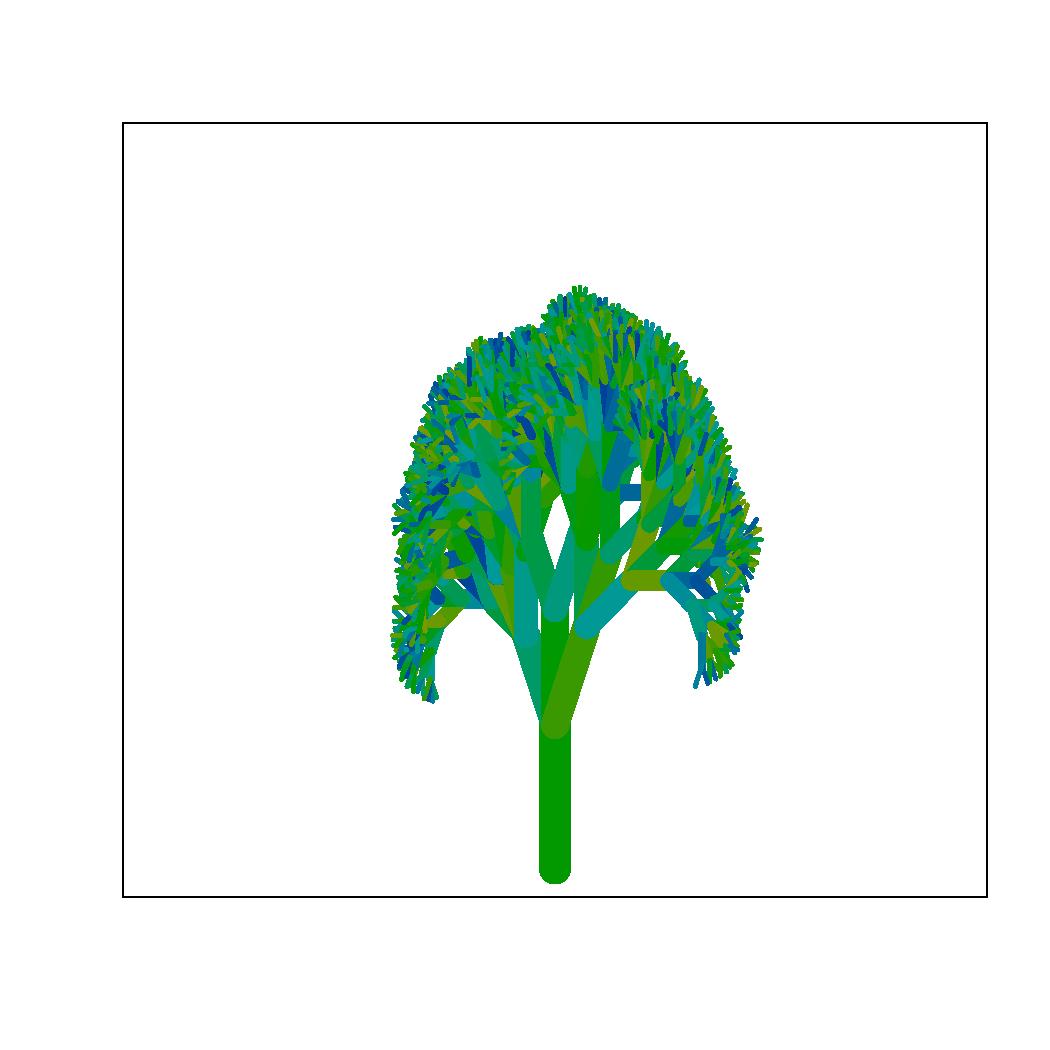
\includegraphics[width=\maxwidth]{figure/unnamed-chunk-13-1} 

\end{knitrout}
\end{Answer}

\begin{Exercise}[difficulty=3, title={Find a mistake in a family tree}]
The file \texttt{wrongpedigree.csv} contains a pedigree (a family tree) containing a mistake: a function we tried to apply on this dataset informed us that the family tree was impossible without more information. We suspect that we have assigned an individual as its own ancestor (this can happen with genetic reconstruction of parentage). Use a self-referencing function to scan the tree and find where the problem is.
\end{Exercise}
\begin{Answer}
I found a solution using two functions: a recursive one, and one going using a for loop to go across incidivuals. Clearly that is not efficient. Feel free to think of a better way!

\begin{knitrout}
\definecolor{shadecolor}{rgb}{0.969, 0.969, 0.969}\color{fgcolor}\begin{kframe}
\begin{alltt}
\hlstd{checkp} \hlkwb{<-} \hlkwa{function}\hlstd{(}\hlkwc{iniind}\hlstd{,} \hlkwc{focalind}\hlstd{,} \hlkwc{ped}\hlstd{,} \hlkwc{level}\hlstd{=}\hlnum{1}\hlstd{,} \hlkwc{maxlevel}\hlstd{=}\hlnum{3}\hlstd{,}
                   \hlkwc{idname} \hlstd{=} \hlstr{"animal"}\hlstd{)}
\hlstd{\{}
  \hlstd{parents} \hlkwb{<-} \hlstd{ped[}\hlkwd{as.character}\hlstd{(ped[,idname])}\hlopt{==}
                   \hlkwd{as.character}\hlstd{(focalind),}\hlkwd{c}\hlstd{(}\hlnum{2}\hlstd{,}\hlnum{3}\hlstd{)]}
  \hlstd{circular} \hlkwb{<-} \hlnum{0}
  \hlkwa{for}\hlstd{(j} \hlkwa{in} \hlnum{1}\hlopt{:}\hlnum{2}\hlstd{)}
  \hlstd{\{}
    \hlkwa{if}\hlstd{(}\hlopt{!}\hlkwd{is.na}\hlstd{(parents[j]))}
    \hlstd{\{}
      \hlkwa{if}\hlstd{(}\hlkwd{as.character}\hlstd{(iniind)}\hlopt{==}\hlkwd{as.character}\hlstd{(parents[j]))}
      \hlstd{\{}
        \hlstd{circular} \hlkwb{<-} \hlstd{circular}\hlopt{+}\hlnum{1}
        \hlkwd{warning}\hlstd{(}\hlstr{"Individual"}\hlstd{, iniind,} \hlstr{" is its own ancestor at level "}\hlstd{,}
                \hlstd{level,}  \hlstr{" (pair "}\hlstd{, parents[}\hlnum{1}\hlstd{],}\hlstr{";"}\hlstd{, parents[}\hlnum{2}\hlstd{],} \hlstr{")"}\hlstd{)}
      \hlstd{\}}\hlkwa{else}\hlstd{\{}
        \hlkwa{if}\hlstd{(level}\hlopt{<}\hlstd{maxlevel)}
        \hlstd{\{level} \hlkwb{<-} \hlstd{level}\hlopt{+}\hlnum{1}
        \hlstd{circular} \hlkwb{<-} \hlstd{circular} \hlopt{+} \hlkwd{checkp}\hlstd{(}\hlkwc{iniind}\hlstd{=iniind,} \hlkwc{focalind}\hlstd{=parents[j],}
                                      \hlkwc{ped} \hlstd{= ped,} \hlkwc{level}\hlstd{=level)}
        \hlstd{\}}
      \hlstd{\}}
    \hlstd{\}}
  \hlstd{\}}
  \hlkwd{return}\hlstd{(circular)}
\hlstd{\}}
\end{alltt}
\end{kframe}
\end{knitrout}

\begin{knitrout}
\definecolor{shadecolor}{rgb}{0.969, 0.969, 0.969}\color{fgcolor}\begin{kframe}
\begin{alltt}
\hlstd{checkpedwrap} \hlkwb{<-} \hlkwa{function}\hlstd{(}\hlkwc{ped}\hlstd{,} \hlkwc{idname}\hlstd{=}\hlstr{"animal"}\hlstd{,} \hlkwc{maxlevel}\hlstd{=}\hlnum{3}\hlstd{)}
\hlstd{\{}
  \hlstd{ped}\hlopt{$}\hlstd{circularity} \hlkwb{<-} \hlnum{NA}
  \hlkwa{for} \hlstd{(i} \hlkwa{in} \hlnum{1}\hlopt{:}\hlkwd{nrow}\hlstd{(ped))}
  \hlstd{\{}
    \hlstd{ped}\hlopt{$}\hlstd{circularity[i]} \hlkwb{<-} \hlkwd{checkp}\hlstd{(}\hlkwc{iniind}\hlstd{=ped[i, idname],}
                                 \hlkwc{focalind} \hlstd{= ped[i, idname],}
                                 \hlkwc{ped}\hlstd{=ped,} \hlkwc{level} \hlstd{=}\hlnum{1}\hlstd{,}
                                 \hlkwc{maxlevel}\hlstd{=maxlevel,} \hlkwc{idname}\hlstd{=idname)}
  \hlstd{\}}
  \hlkwd{return}\hlstd{(ped)}
\hlstd{\}}
\end{alltt}
\end{kframe}
\end{knitrout}


\begin{knitrout}
\definecolor{shadecolor}{rgb}{0.969, 0.969, 0.969}\color{fgcolor}\begin{kframe}
\begin{alltt}
\hlstd{ped} \hlkwb{<-} \hlkwd{read.csv}\hlstd{(}\hlstr{"wrongpedigree.csv"}\hlstd{,} \hlkwc{stringsAsFactors} \hlstd{=} \hlnum{FALSE}\hlstd{)}
\hlstd{pedchecked} \hlkwb{<-} \hlkwd{checkpedwrap}\hlstd{(}\hlkwc{ped}\hlstd{=ped,} \hlkwc{idname} \hlstd{=} \hlstr{"animal"}\hlstd{,} \hlkwc{maxlevel} \hlstd{=} \hlnum{3}\hlstd{)}
\end{alltt}


{\ttfamily\noindent\color{warningcolor}{\#\# Warning in checkp(iniind = iniind, focalind = parents[j], ped = ped, level = level): IndividualCN15-053 is its own ancestor at level 3 (pair CN15-F7;CN15-053)}}\end{kframe}
\end{knitrout}
\end{Answer}


\end{document}
